\section{Evaluation}
\label{sec-evaluation}

We continue by demonstrating that our \PocketMocker{} prototype works by using
it to mock three smartphone apps. In each case we describe the app, discuss why
users might want to mock it, describe our specific mocking objective and
whether it was achieved.

\subsection{Mocking Maps}

\begin{figure*}[t]

\begin{subfigure}[t]{0.33\textwidth}
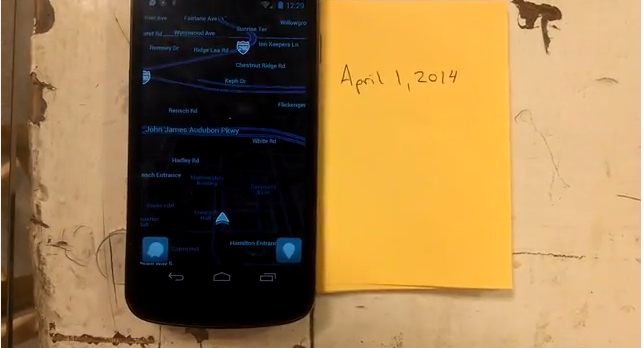
\includegraphics[width=\textwidth]{./figures/apps/waze/waze1.png}
\caption{}
\end{subfigure}%
\begin{subfigure}[t]{0.33\textwidth}
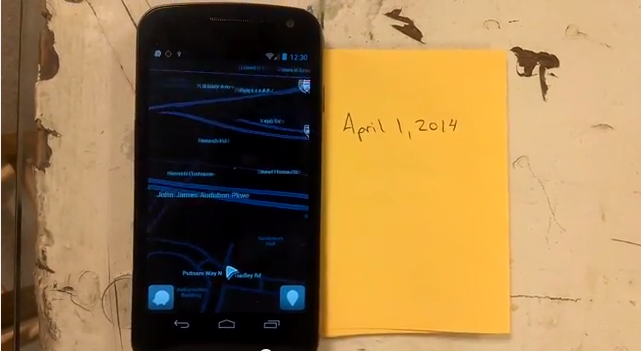
\includegraphics[width=\textwidth]{./figures/apps/waze/waze2.png}
\caption{}
\end{subfigure}%
\begin{subfigure}[t]{0.33\textwidth}
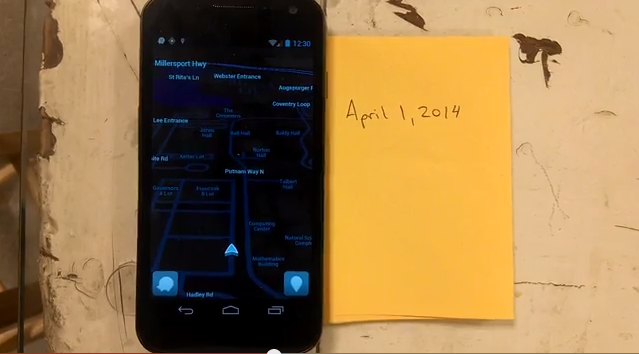
\includegraphics[width=\textwidth]{./figures/apps/waze/waze3.png}
\caption{}
\end{subfigure}%

\caption{\textbf{Mocking Waze.} The screenshots demonstrate that we were
successfully able to mock the Waze maps app. As the mocking trace is
replayed, the phone remains stationary on the desk, but Waze thinks that the
user is walking around.}

\vspace*{0.1in}
\hrule
\vspace*{-0.15in}

\label{fig-mocking-waze}

\end{figure*}

As a first example of \PocketMocker{} in action, we mock the Waze maps
app~\cite{waze-playstore-url}. Waze describes itself as a community-based
traffic and navigation app allowing ``millions of drivers from across the
globe joining forces to outsmart traffic, save time, gas money, and improve
daily commuting for all''.

Our objective in mocking Waze was to show that \PocketMocker{} can provide
fine-grained location to the many smartphone apps that use location to
customize the user experience. Given the amount of information smartphone
users' location can reveal about them, it is important for \PocketMocker{} to
effectively support location mocking. In our next mocking example we show the
effect that mocked locations can have on an unsuspecting app.

To mock Waze, We first recorded a mocking trace of a walk around campus,
described in more detail in Table~\ref{table-mocking-waze}.  This included
tracking location, connectivity, and sensor data from the gyroscope and
accelerometer that Waze utilizes. We then placed the smartphone on a desk,
initiated a replay session and launched the Waze app.
Figure~\ref{fig-mocking-waze} shows three screenshots of Waze being mocked,
showing that the users location is being updated to follow the trace despite
the smartphone not moving. An anonymized video of our successful Waze mocking
session is also available at
\hyperlink{http://youtu.be/GIqXP6b769c}{\texttt{http://youtu.be/GIqXP6b769c}}.

\begin{table}
\begin{tabularx}{3.33in}{lX}
\textbf{App} & Waze Social Maps \& Traffic \\ \toprule
\textbf{Installs} & 10--50~million \\
\textbf{Mocking Objective} & Mock location \\ \midrule
\textbf{Trace Length} & 2 minutes 27 seconds \\
\textbf{Trace Size} & 516~K \\
\textbf{Location Mocks} & 117 \\
\textbf{Sensors Used} & {\small GPS, Gyroscope, Accelerometer} \\
\textbf{Sensor Mocks} & 2773 \\
\textbf{Wifi Scan Mocks} & 115 \\
\textbf{Cell Location Mocks} & 117 \\
\textbf{Video URL} &
\hyperlink{http://youtu.be/GIqXP6b769c}{\texttt{http://youtu.be/GIqXP6b769c}} \\

\end{tabularx}

\caption{\textbf{Mocking Waze.} Details of our Waze mocking trace.}

\label{table-mocking-waze}

\end{table}

\subsection{Mocking Checkins}

As an example of a more realistic mocking scenario, we used \PocketMocker{}
to mock the popular Facebook app~\cite{facebook-playstore-url}. Facebook is
the world's largest social networking site and its Android app is quite
popular, with the Play Store estimating between 500~million and 1~billion
installs. People use Facebook to share content and stay in touch with
friends.

Our objective in mocking Facebook was to initiate a check-in at a mocked
location. Facebook check-ins are shared with friends (and advertisers), so a
user may want to create a fraudulent check-in for many reasons. It could be
health-related, like our Alice, so different ads are displayed when the user
visits the website, or it could be reputation-related as a user may want to
appear more social than he or she really is.

To mock a Facebook check-in, we recorded a mocking trace of a walk to the
nearby Starbucks, which included location, connectivity, and sensor data from
the accelerometer. Because the trace was collected outdoors, no Wifi scan
data was captured. We then placed the smartphone on a desk, initiated a
replay session and launched the Facebook app.

Figure~\ref{fig-mocking-facebook} shows three screenshows of Facebook being
mocked demonstrating that Facebook did allow us to check in at Starbucks at
the end of the trace despite the smartphone not being located nearby. We did
record a video of the mocking process, but due to the amount of personal
information revealed by Facebook we were not able to anonymize it
sufficiently.

\begin{figure*}[t]

\begin{subfigure}[t]{0.33\textwidth}
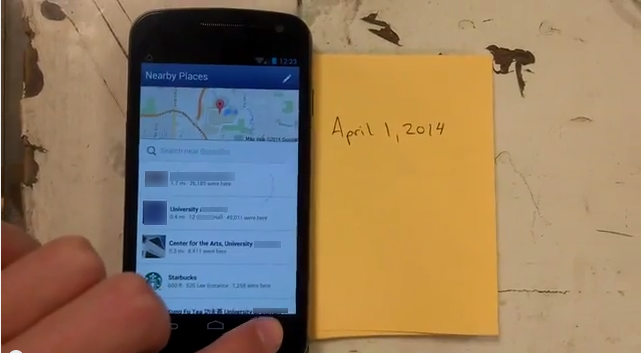
\includegraphics[width=\textwidth]{./figures/apps/facebook/facebook1.png}
\caption{}
\end{subfigure}%
\begin{subfigure}[t]{0.33\textwidth}
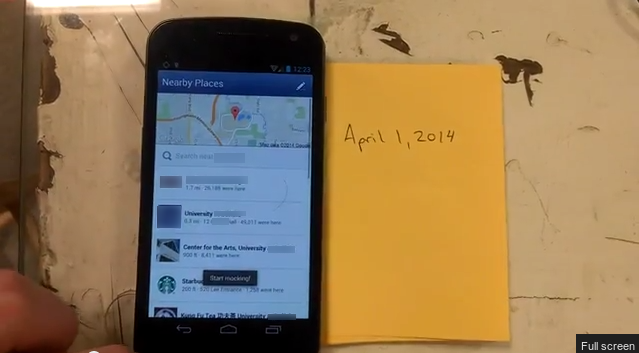
\includegraphics[width=\textwidth]{./figures/apps/facebook/facebook2.png}
\caption{}
\end{subfigure}%
\begin{subfigure}[t]{0.33\textwidth}
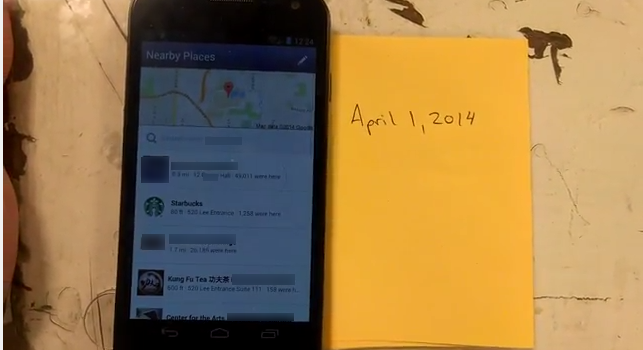
\includegraphics[width=\textwidth]{./figures/apps/facebook/facebook3.png}
\caption{}
\end{subfigure}

\caption{\textbf{Mocking Facebook.} The screenshots show that we were able to
mock the Facebook app and initiate a check-in at Starbucks from a half-mile
away.}

\vspace*{0.1in}
\hrule
\vspace*{-0.15in}

\label{fig-mocking-facebook}

\end{figure*}

\begin{table}[t]
\begin{tabularx}{3.33in}{lX}
\textbf{App} & Facebook \\ \toprule
\textbf{Installs} & 500--1,000~million \\
\textbf{Mocking Objective} & Check-in at mocked location. \\
  \midrule
\textbf{Trace Length} & 1 minute 37 seconds \\
\textbf{Trace Size} & 268~K \\
\textbf{Location Mocks} & 106 \\
\textbf{Uses Sensors} & GPS, Accelerometer \\
\textbf{Sensor Mocks} & 2569 \\
\textbf{Wifi Scan Mocks} & 0 \\
\textbf{Cell Location Mocks} & 97 \\
\textbf{Video URL} & 
\hyperlink{http://youtu.be/R8L6OV8hY2k}{\texttt{http://youtu.be/R8L6OV8hY2k}} \\

\end{tabularx}

\caption{\textbf{Mocking Facebook.} Details of our Facebook mocking trace.}

\label{table-mocking-facebook}

\end{table}

\subsection{Mocking a Game}

As a final mocking challenge, we attempted to use \PocketMocker{} to mock an
accelerometer-driven game. Fast Racing 3D is a car racing game available for
Android~\cite{fastracing-playstore-url}. Gaming is a popular activity on
smartphones, with studies showing that 32~\% of time spent on smartphones
being devoted to game play~\cite{flurry-smartphoneuse}. While \PocketMocker{}
normally records sensor data aggressively during recording in order to ensure
that it collects a superset of any information that could be requested during
the mocking session, games provide a particular challenge for replay due to
their aggressive use of high-rate sensor data---in this case, the
accelerometer.

Our objective in mocking Fast Racing was to use the mocked trace to control
gameplay during the mocking session. Users may want to mock apps for several
reasons: to avoid tedious replay of easier levels on apps that force players
to begin again after failing more difficult challenges, or to improve their
reputation through repetition when using apps that post scores to a public
leaderboard.

To mock Fast Racing gameplay we recorded a mocking trace of a portion of a
trip through one of the game's race courses.  This included tracking location,
connectivity, as well as sensor data from the accelerometer used to control
the vehicle. We then placed the smartphone on a desk, launched the Fast
Racing app, and initiated trace replay. Figure~\ref{fig-mocking-game} shows
three screenshots of Fast Racing being mocked demonstrating that the
accelerometer data was able to control the Fast Racing vehicle. For this
particular scenario, however, we found it difficult to trigger the mocking
replay at precisely the correct moment, with the associated time delay
causing the vehicle's path to eventually deviate from the original trace as
the mocking session continued. An anonymized video of our semi-successful
Fast Racing mocking session is also available at
\hyperlink{http://youtu.be/8fAj5dYFwS0}{\texttt{http://youtu.be/8fAj5dYFwS0}}.

\begin{figure*}[t]

\begin{subfigure}[t]{0.33\textwidth}
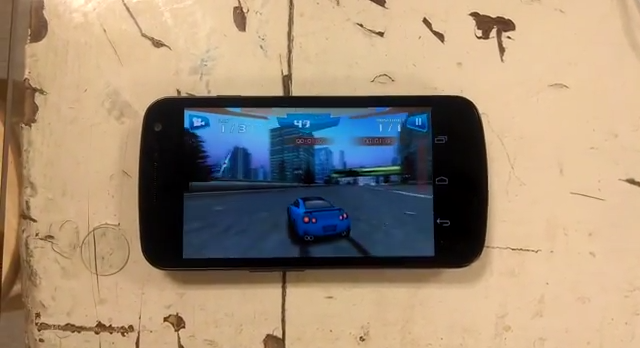
\includegraphics[width=\textwidth]{./figures/apps/fast_racing/fastracing1.png}
\caption{}
\end{subfigure}%
\begin{subfigure}[t]{0.33\textwidth}
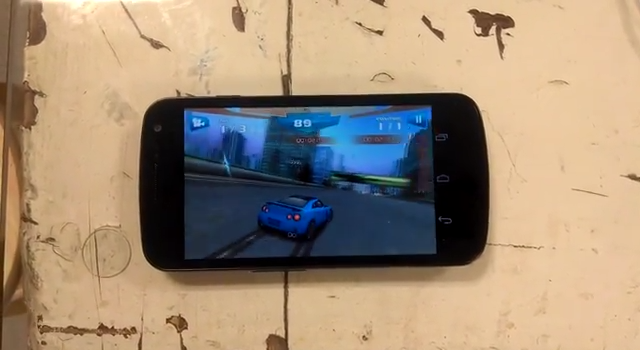
\includegraphics[width=\textwidth]{./figures/apps/fast_racing/fastracing2.png}
\caption{}
\end{subfigure}%
\begin{subfigure}[t]{0.33\textwidth}
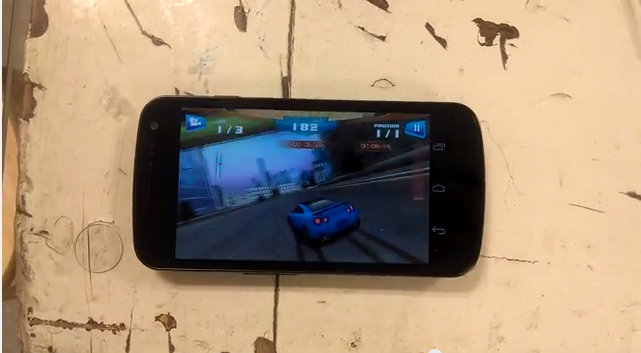
\includegraphics[width=\textwidth]{./figures/apps/fast_racing/fastracing3.png}
\caption{}
\end{subfigure}

\caption{\textbf{Mocking Fast Racing.} The screenshots show that we were able
to mock the accelerometer-driven Fast Racing game.}

\vspace*{0.1in}
\hrule
\vspace*{-0.15in}

\label{fig-mocking-game}

\end{figure*}

\begin{table}[t]

\begin{tabularx}{3.33in}{lX}
\textbf{App} & Fast Racing 3D \\ \toprule
\textbf{Installs} & 50--100~million \\
  \textbf{Mocking Objective} & Control game play \\ \midrule
\textbf{Uses Sensors} & Accelerometer \\
\textbf{Trace Length} & 1 minute 35 seconds \\
\textbf{Trace Size} & 296~K \\
\textbf{Location Mocks} & 96 \\
\textbf{Uses Sensors} & GPS, Accelerometer \\
\textbf{Sensor Mocks} & 1363 \\
\textbf{Wifi Scan Mocks} & 96 \\
\textbf{Cell Location Mocks} & 96 \\
\textbf{Video URL} &
  \hyperlink{http://youtu.be/8fAj5dYFwS0}{\texttt{http://youtu.be/8fAj5dYFwS0}}
  \\

\end{tabularx}

\caption{\textbf{Mocking Fast Racing.} Details of our Fast Racing
  mocking trace.}

\label{table-mocking-game}
\vspace*{-0.2in}
\end{table}


\subsection{Users Can Use \PocketMocker{}}
\label{subsec-usability}

% 03 Apr 2014 : GWA : ND TODO : 1 column (0.5 page) about the experiment.
% Describe the app, what it does, how many people participated, etc. Then
% some bits of the qualitative feedback.

With a  prototype implemented, we wanted to gain a qualitative insight to
future users of \PocketMocker{}. Over the course of one day, we had 7 users use
our most recent record-and-replay prototype. Due to physical limitations, we
studied users individually with one Galaxy Nexus smartphone. 

After receiving some background information on the project and instructions
on how to use \PocketMocker{}, users were given the smartphone with the goal
of tricking an open-source Pedometer~\cite{pedometer-playstore-url} that they
were walking (and being active beings), while the phone was sitting on the
desk in the lab. We wanted to receive feedback on the app, the idea,
and the process, so we collected responses to the following questions after
they saw \PocketMocker{} in action: ``Did \PocketMocker{} mock the Pedometer?'' and
``Comments?''. All users reacted positively, with one who ``would love to use
it for some other apps'' and 42\% of our users believe it has strong
``potential''. 

The users found the app and process to be extremely transparent: all
that was needed was to open the app, create an objective, hit record, and
forget about it. In all cases, \PocketMocker{} was able to trick the
Pedometer into classifying the phone's action as walking---by showing steps
increase---when the phone was really sitting idle on a desk.
